% !TEX root = ../YourName-Dissertation.tex

\chapter{Neutrinos and Neutrino Masses}

\section{Introduction}



\section{Neutrinos}

The neutrino was first hypothesized by Dirac to explain the observation that beta-decay radiation is emitted in a continuous spectrum rather than a monoenergetic peak. Neutrinos, Italian for "little neutral one", were little more than a speculation when first hypothesize, so it is rather remarkable that neutrinos were eventually discovered by the work of Reines and Cowan in the 20th century. 

While first discovered in the context of nuclear physics, neutrinos have a pervasive presence throughout our universe. Not only are neutrinos important for our understanding of nuclear processes, but also to our understanding of cosmology and particle physics. It is fitting that the most abundant fermion in our universe should play a fundamental role in our understanding of the universe at is largest and smallest scales.

\section{Neutrino Oscillations}

Back in the day the solar neutrino problem was noticed in the experiment by Ray Davis. Neutrinos from the sun were missing. The experiment took place at the Sanford mine in South Dakota.

Neutrino oscillations were first observed by the Super-Kamiokande (SK) experiment in th 90's. The rates of atmospheric neutrinos from above and below were compared.

Neutrino oscillations were independently confirmed by the Sudbury Neutrino Observatory experiment (SNO) using solar neutrinos. 

Both experiments were awarded the Nobel prize in 2015 for the discover of neutrino oscillations.

Today the number of experiments which have measured rates of neutrino oscillation are legion. Measurements have been performed using various sources of neutrinos such as nuclear reactor, solar, atmospheric, and accelerator. 

The origin of neutrino oscillations is that the weak eigenstates are distinct from the mass eigenstates. The weakly interacting eigenstates are described as a superposition of the massive neutrino states using a 3x3 mixing matrix. 

The neutrino mixing matrix is typically written in the Pontecorvo-Maki-Nakagawa-Sakata (PMNS) parameterization.

\begin{figure}[htbp]
    \centering
    \includegraphics[width=0.6\textwidth]{figs/Chapter-2/230227_chap2_nu_hierarchy.png}
    \caption{Caption}
    \label{fig:chap2-nu-hierarchy}
\end{figure}

A giant experimental effort over the past couple of decades has greatly contained the majority of parameters in the PMNS matrix, many to relative uncertainties of only a few percent. However, some parameters still remain relatively unconstrained, which is the origin of the current uncertainty in the ordering of the neutrino masses. Next-generation neutrino oscillation experiments such as JUNO, Hyper-Kamiokande, and DUNE are poised to resolve this ambiguity in the coming years.

As one can see from the equation for neutrino mixing probabilities, the dependence on mass only enters as a difference between the mass eigenstates. Therefore oscillation probabilities are unaffected by the absolute scale of the neutrino mass. However, oscillations can be used to obtain a lower bound on the neutrino masses by setting the mass of the lightest neutrino mass state to zero. This results in different lower limits depending on the ordering of the neutrino mass states.

\begin{figure}[htbp]
    \centering
    \begin{subfigure}{0.7\textwidth}
        \includegraphics*[width=\textwidth]{figs/Chapter-2/230302_mass_estate_vals_normal.png}
        \caption{}
    \end{subfigure}
    \hfill
    \begin{subfigure}{0.7\textwidth}
        \includegraphics*[width=\textwidth]{figs/Chapter-2/230302_mass_estate_vals_inverted.png}
        \caption{}
    \end{subfigure}
    \caption{Caption}
    \label{fig:chap2-mass-estates}
\end{figure}

Various extensions to the 3x3 mixing regime, so called sterile neutrinos, have been proposed to explain certain anomalous neutrino oscillation phenomena observed primarily in neutrinos produced by nuclear reactors. Currently there is inconclusive evidence to support the existence of sterile neutrinos. Certain of these apparently anomalous results can be explained by better modeling of the nuclear processes in the reactors that generate the measured flux of neutrinos. However, some puzzles such as the unexplained neutrino deficits measured by the BEST experiment remain open.  

\section{Neutrino Masses in the Standard Model}

In modern quantum field theory spin-1/2 particles, or Fermions, are described using the Dirac equation. 

Fermion masses in the standard model are a result of the Higgs mechanism, which requires both left-chiral and right-chiral fermion fields. The current experimental evidence for neutrinos only support the existence of right-handed neutrinos and left-handed antineutrinos, therefore, neutrinos in the standard model are predicted to have zero mass. Consequently, the observation of neutrino oscillations is inconsistent with the standard model.

Since neutrinos are neutral particles, the simplest extension to the standard model is to allow neutrinos to have a Majorana mass term of the form \ldots If neutrinos are indeed Majorana fermions then one would predict that certain nuclei can decay via the rare neutrino-less double-beta decay process at a rate proportional to the neutrino mass absolute scale. 

Alternatively, if neutrinos are instead Dirac Fermions, one can generate neutrino masses in the standard model by allowing the existence of right-handed neutrino states. In this case neutrino masses are generated in the same way as other Fermions through the Yukawa coupling terms of the form \ldots These right-handed neutrino states are disallowed from interacting with the rest of the standard model other than gravitationally in order to be consistent with experimental data and are thus often referred to as "sterile neutrinos" due to their lack of weak interactions. Despite their lack of weak interactions it is possible for sterile neutrinos to be observed via their effects on neutrino oscillations.

These simple extensions to the standard model are dissatisfactory to many physicist, since they require coupling constants to the Majorana and Yukawa mass terms that are many orders of magnitude smaller than other fermions in order to generate neutrino masses consistent with observation data. The absolute masses of neutrinos are on the order of $10^{-6}$ smaller than the electron, which is suggestive that the origin of neutrino masses is the result of some new physics beyond the standard model.

A popular extension to the standard model to explain the smallness of the neutrino mass is the so-called see-saw mechanism \ldots

\section{Neutrino Absolute Mass Scale}

Neutrino oscillation probabilities are determined by the squared mass differences and are insensitive to the absolute neutrino mass scale, therefore, alternative probes are needed to perform an effective measurement of the neutrino mass.

\subsection{Limits from Cosmology}

In the $\Lambda$CDM model, which summarizes our current cosmological understanding of our universe, the mass-energy content of the universe is composed of approximately 27\% dark matter and only 5\% normal matter including neutrinos. From this observation, a rough limit on the neutrino mass can be obtained from the condition that neutrinos are not responsible for the entirety of the matter content of the universe. Using only this condition one can constrain the neutrino mass to be \ldots

A prediction of the $\Lambda$CDM model is that the universe originated from a single expansion event colloquially called the "Big Bang". In the Big Bang scenario, out universe originated as a hot spacetime singularity, which abruptly experience rapid expansion in a process called inflation. After the inflationary epoch the universe entered the reheating phase where the potential energy responsible for inflation decays into standard model particles such as electrons, quarks, and gluons. The universe continued to expand in size resulting in a decrease in energy density and lower temperature. Eventually the temperature of the universe decreased enough 

\begin{figure}[htbp]
    \centering
    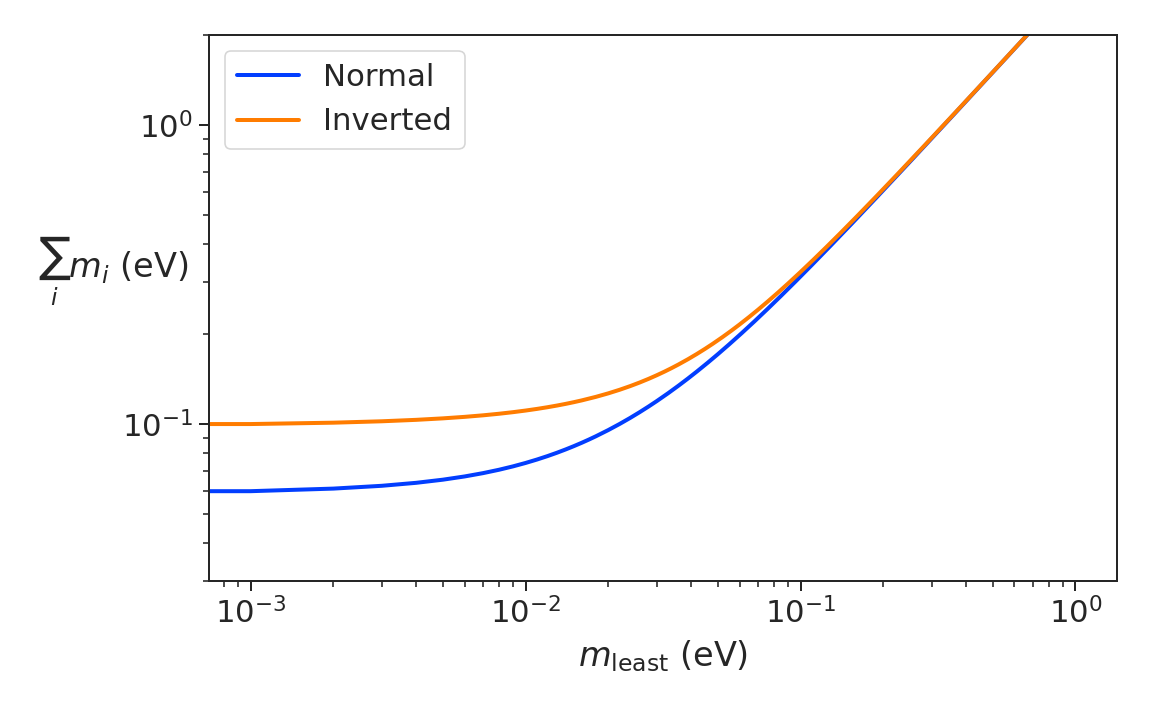
\includegraphics[width=0.7\textwidth]{figs/Chapter-2/230301_cosmology_nu_mass_observable.png}
    \caption{Caption}
    \label{fig:nu_mass_cosmo}
\end{figure}


\subsection{Limits from Neutrinoless Double Beta-decay Searches}

\begin{figure}[htbp]
    \centering
    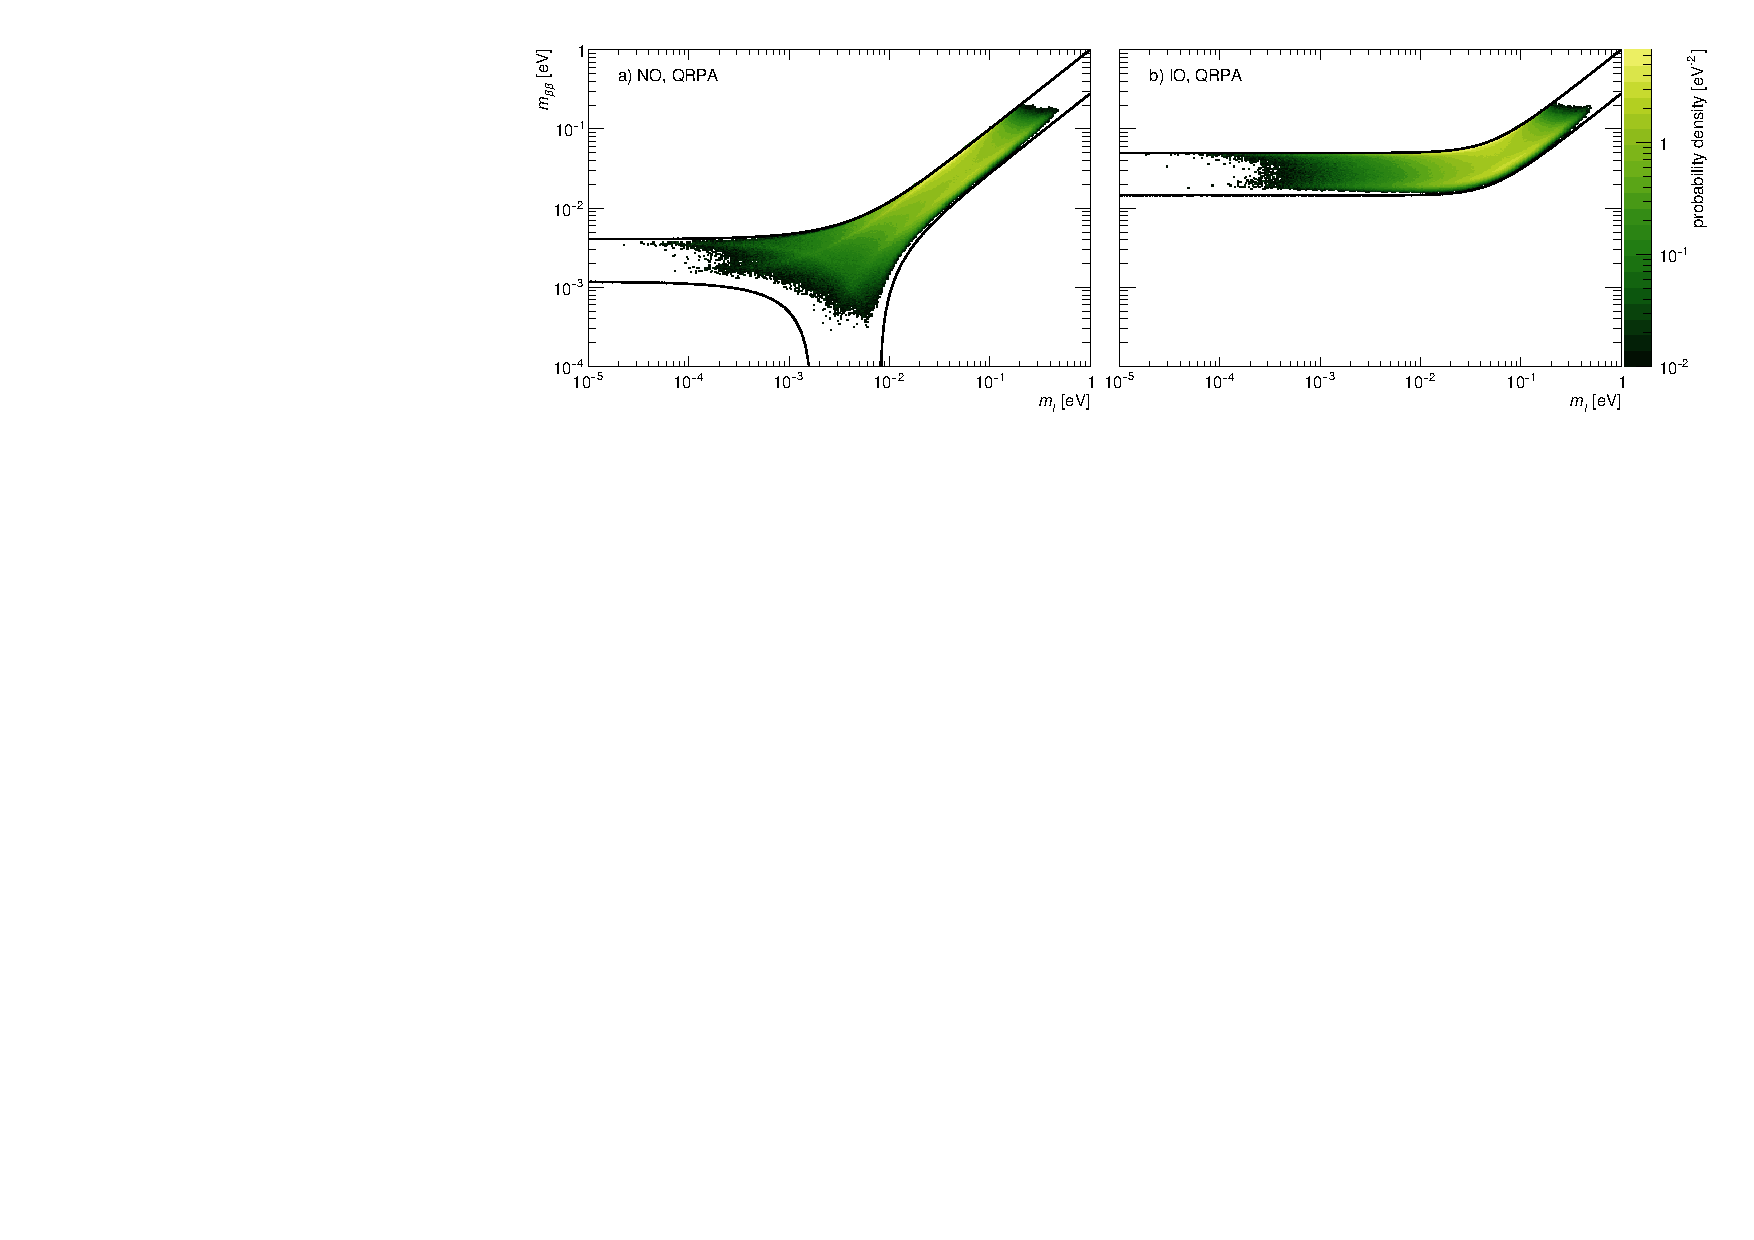
\includegraphics[width=1.0\textwidth]{figs/Chapter-2/230228_nu_mass_0nbb.pdf}
    \caption{Caption}
    \label{fig:nu_mass_0nbb_posterior}
\end{figure}

\begin{figure}[htbp]
    \centering
    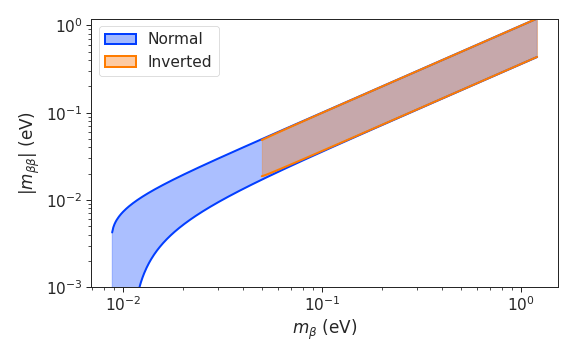
\includegraphics[width=0.7\textwidth]{figs/Chapter-2/230301_mbb_vs_mb.png}
    \caption{Caption}
    \label{fig:nu_mass_0nbb_vs_nu_beta}
\end{figure}

\subsection{Kinematic Measurements of the Neutrino Mass}

\begin{figure}[htbp]
    \centering
    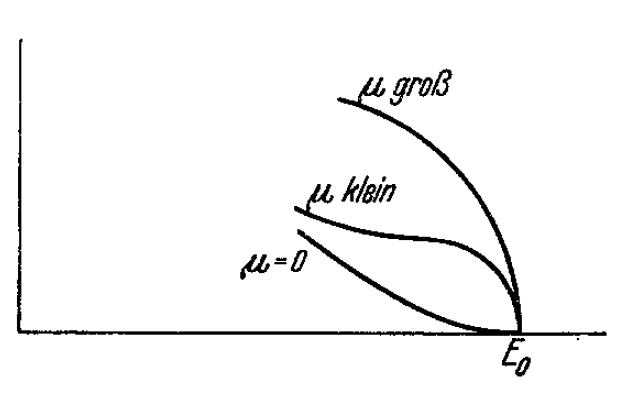
\includegraphics[width=0.7\textwidth]{figs/Chapter-2/Fermi.png}
    \caption{Caption}
    \label{fig:fermi_original_b_spectrum}
\end{figure}

\begin{figure}[htbp]
    \centering
    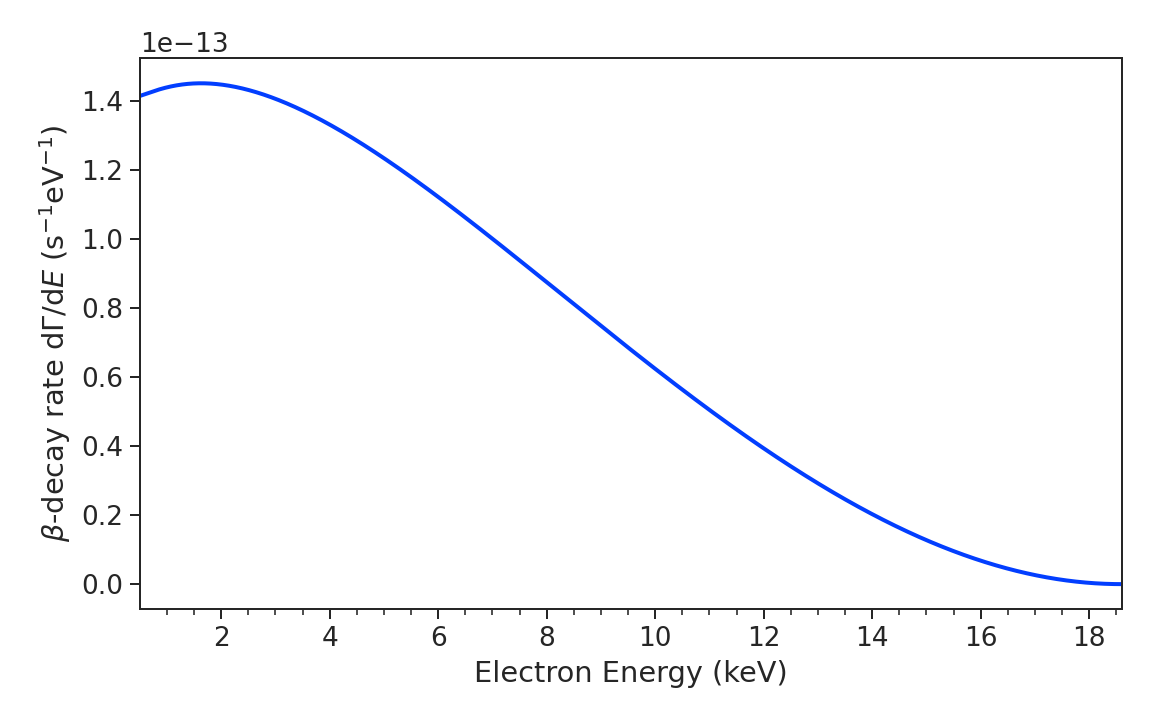
\includegraphics[width=0.7\textwidth]{figs/Chapter-2/230302_atomic_tritium_spectrum.png}
    \caption{Caption}
    \label{fig:atomic_tritium_spectrum}
\end{figure}

\begin{figure}[htbp]
    \centering
    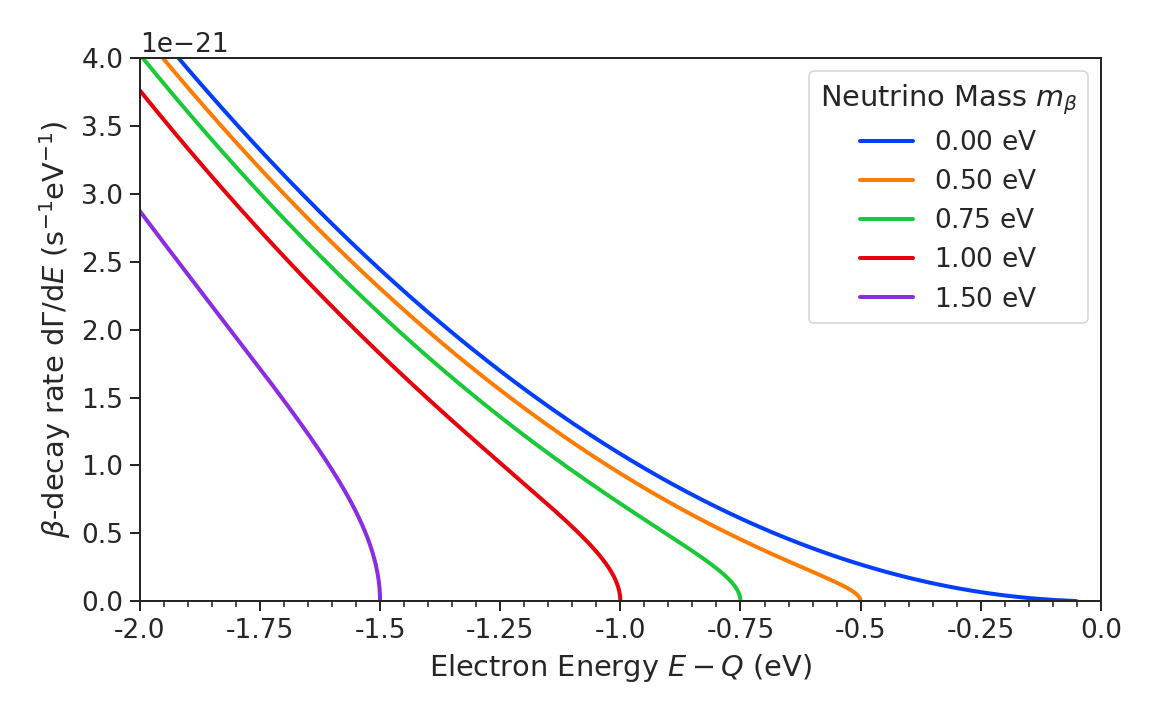
\includegraphics[width=0.7\textwidth]{figs/Chapter-2/230302_atomic_tritium_spectrum_near_endpoint.png}
    \caption{Caption}
    \label{fig:atomic_tritium_endpoint}
\end{figure}
